\section{Resultados}

Logramos consolidar un prototipo de robot omnidireccional ilustrado en la figura \ref{fig:robotfinal}. La estructura cuenta con un sistema de control compensado para el robot, un mapa estructurado gobernado por un conjunto red de Petri/Monitor, una interfaz de usuario con monitoreo y supervisión de las operaciones del robot, además de un Filtro de Kalman para mejorar la precisión en la estimación de la posición del mismo y un mecanismo para medir distancia por medio de códigos QR. Toda esta integración queda reflejada en el diagrama de componentes del sistema de la figura \ref{fig:integsistemadiagcomp}.

\begin{figure}[htpb]
    \centering
    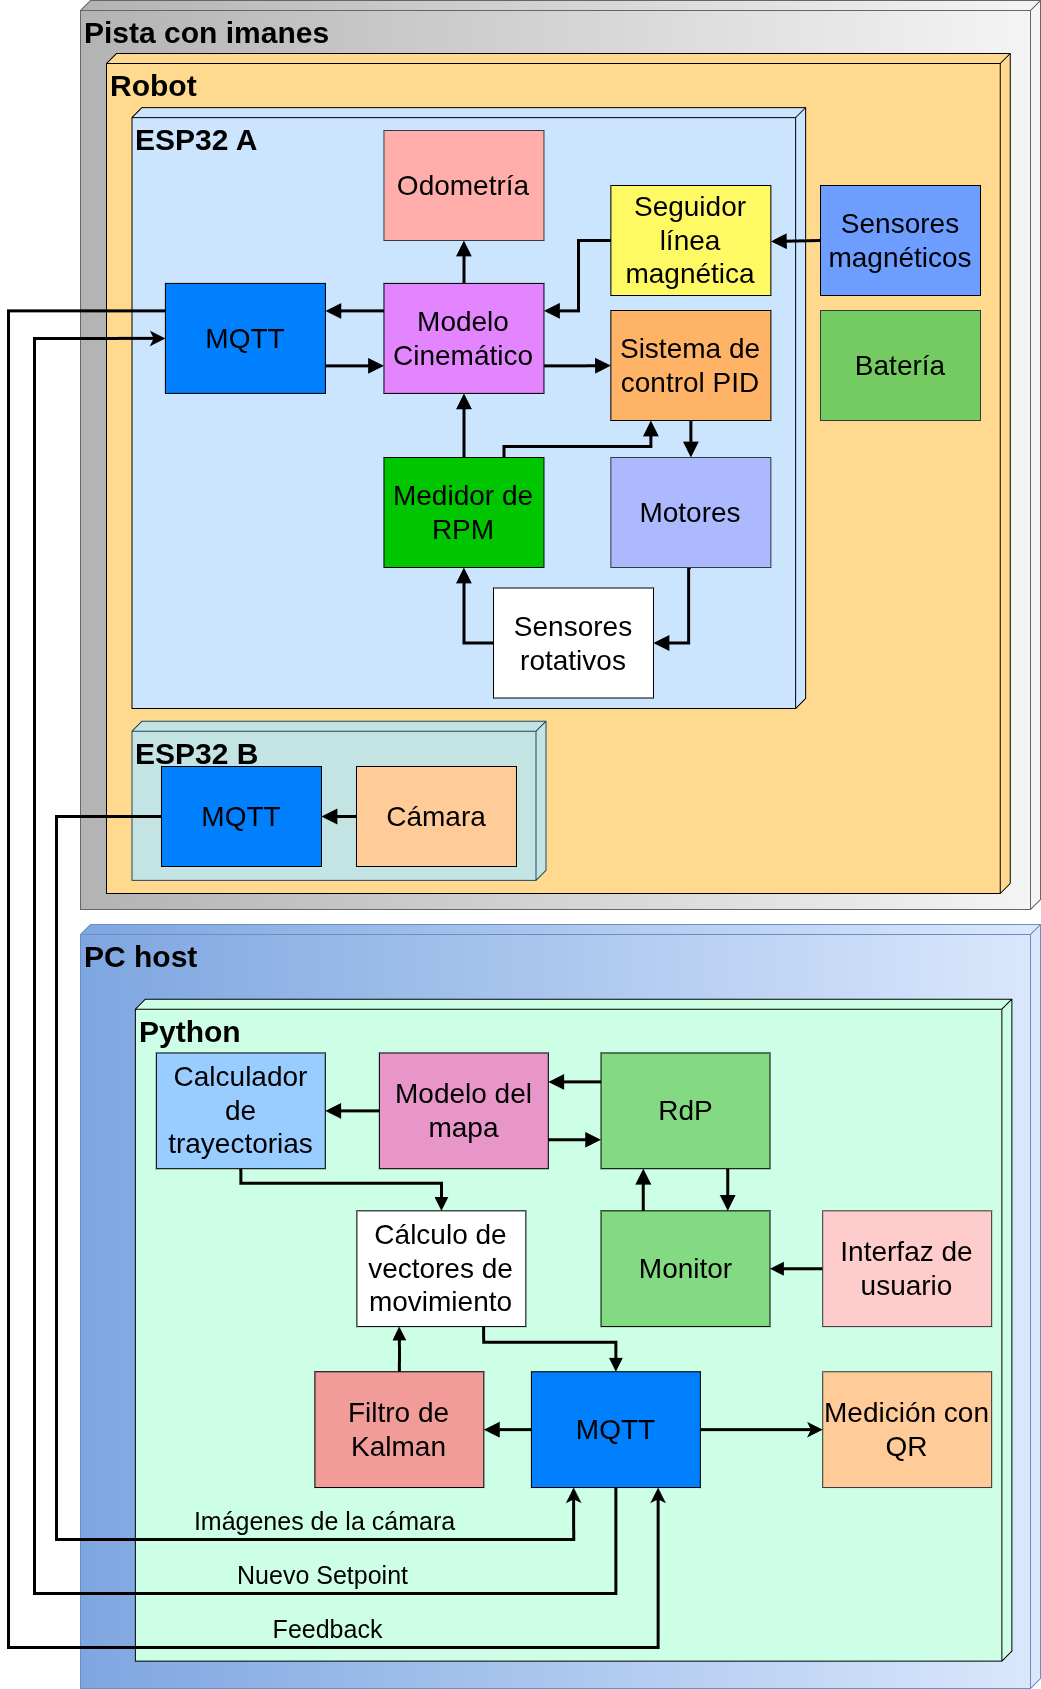
\includegraphics[width=1.0\linewidth]{images/integ_sistema_diag_componentes_vertical.png}
    \caption{Diagrama de componentes del sistema}
    \label{fig:integsistemadiagcomp}
\end{figure}

\begin{figure}[htpb]
    \centering
    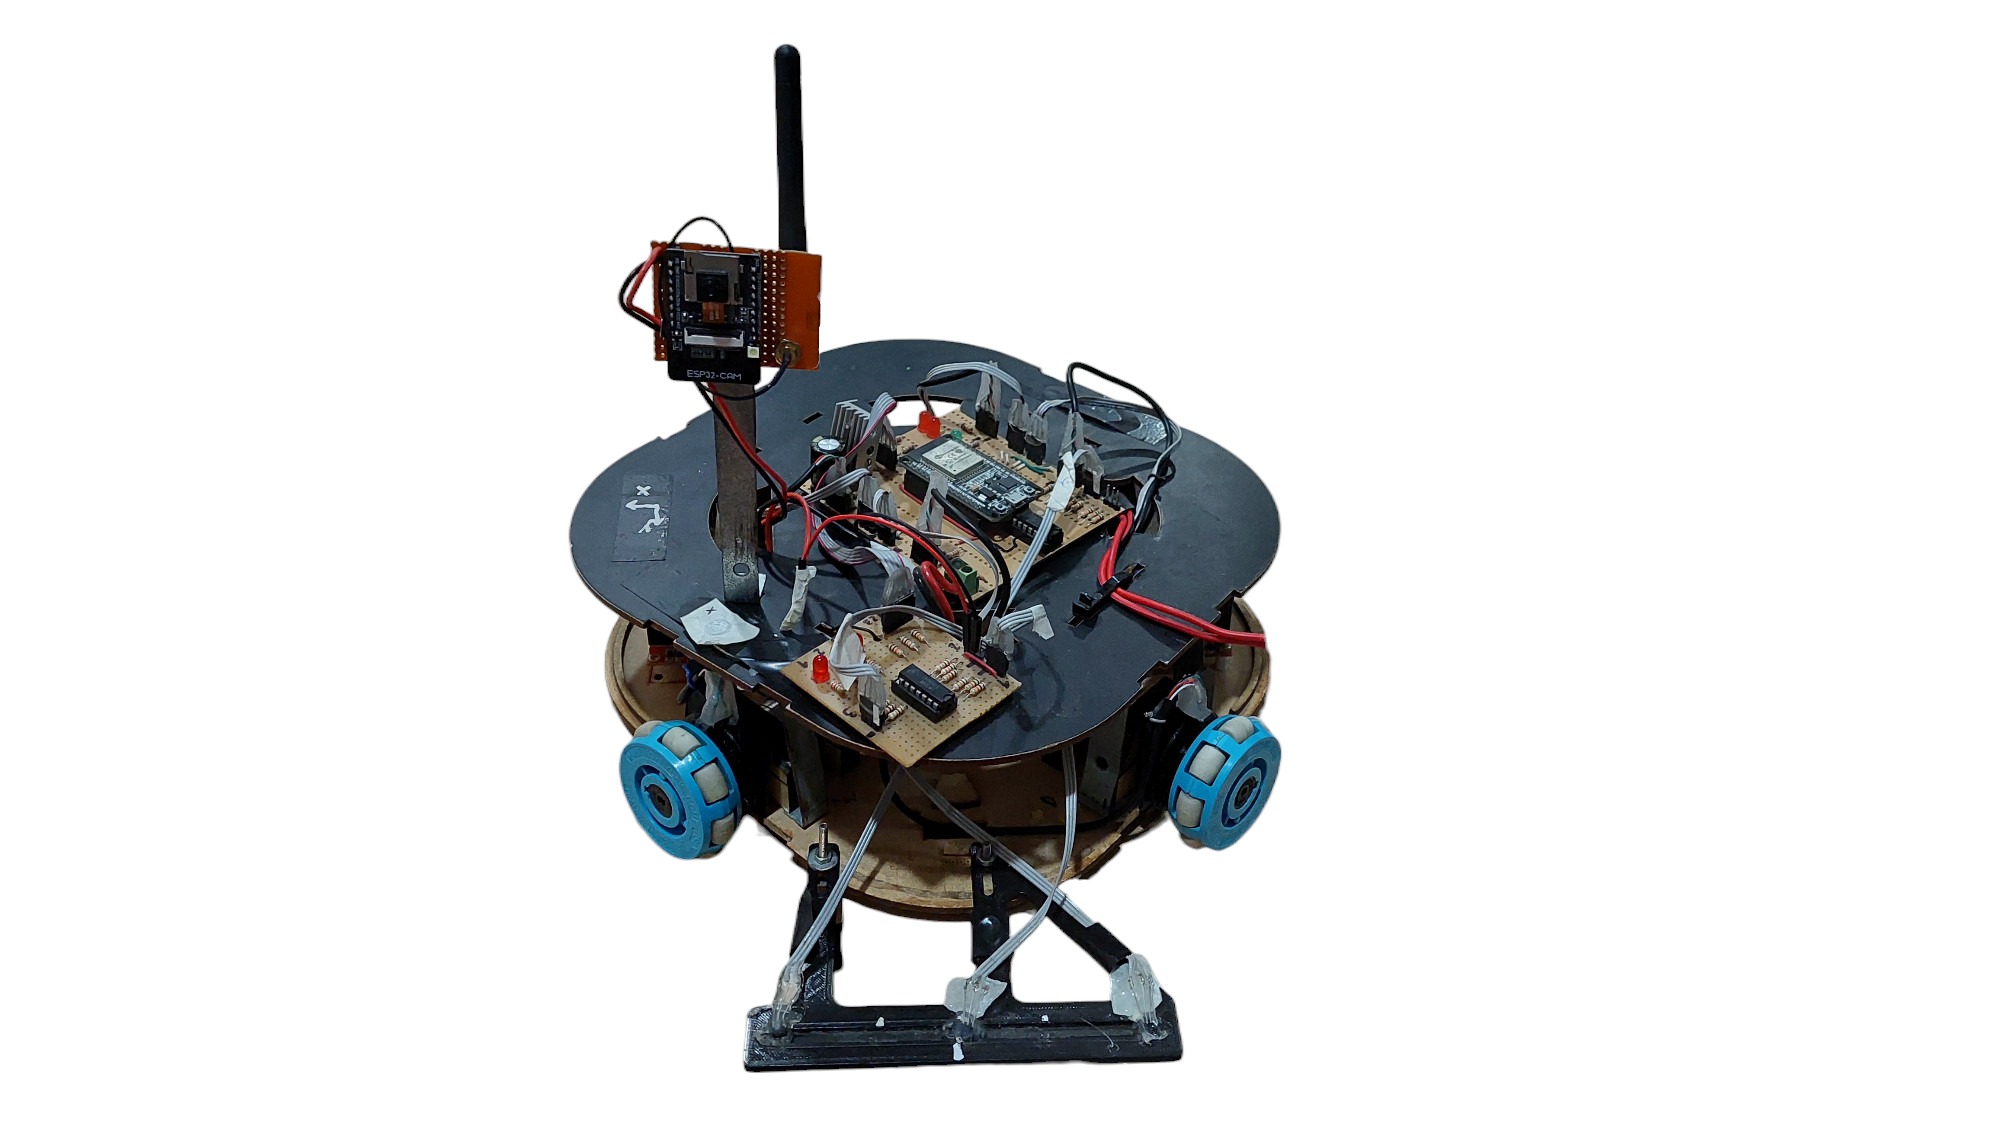
\includegraphics[trim={20cm 1.5cm 20cm 1.5cm}, clip, width=0.6\linewidth]{images/robot_camara.png}
    \caption{Prototipo final del robot con cámara incorporada}
    \label{fig:robotfinal}
\end{figure}

Resulta evidente que en nuestro proyecto integramos múltiples mecanismos para lograr que el movimiento del robot sea lo más efectivo posible. En diferentes niveles, cada sistema de compensación actúa sobre la señal que recibe cada rueda al realizar movimientos. De menor a mayor en nivel de jerarquía, tenemos:

\begin{itemize}
    \item Sistema de control PID por cada rueda.
    \item Modelo cinemático compensado.
    \item Seguidor de línea magnético.
    \item Filtro de Kalman compensado.
\end{itemize}

Por otra parte, en la Figura \ref{fig:integsistemarobotpistaqr} ilustramos cómo el robot interactúa con el resto de los elementos para lograr la funcionalidad completa. El robot está colocado en la pista con imanes, donde el vano central corresponde al obstáculo representado en la interfaz del mapa y es un lugar no transitable. En el mismo espacio están los códigos QR a una altura adecuada en puntos estratégicos para que el robot los lea en puntos clave del mapa.

\begin{figure}[htpb]
    \centering
    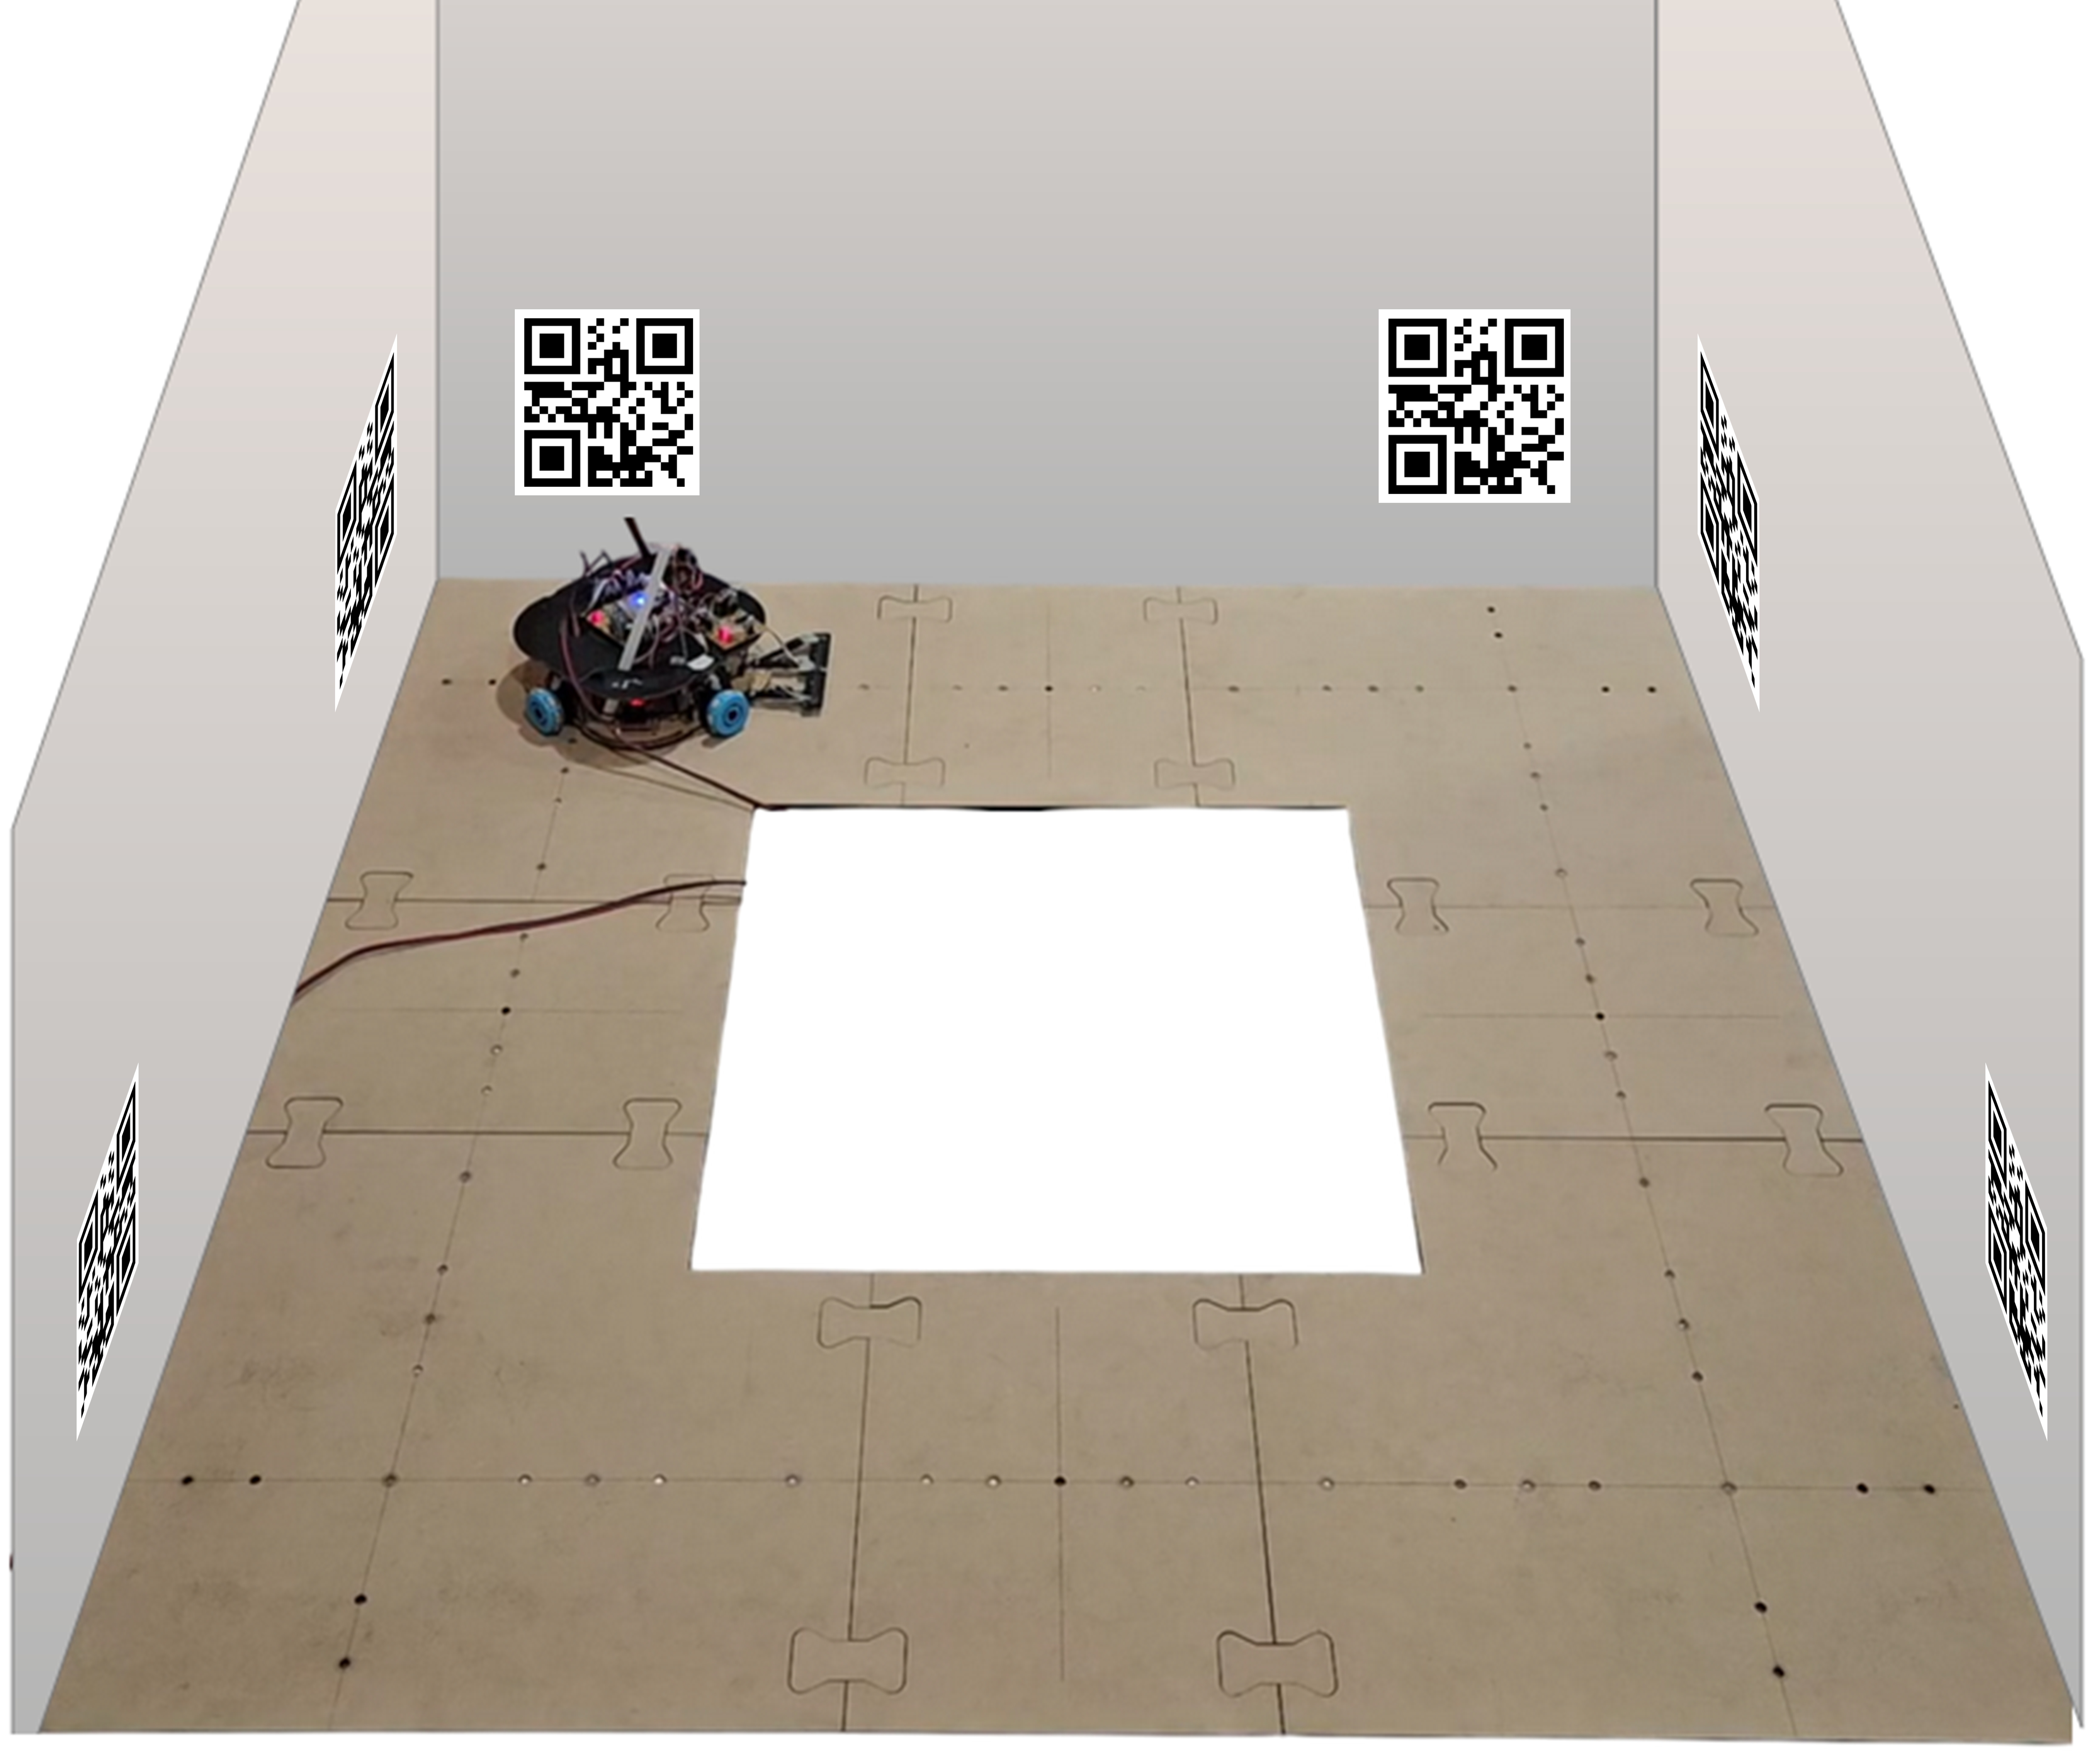
\includegraphics[width=0.9\linewidth]{images/integ_sistema_robot_en_plano.png}
    \caption{Robot en la pista con imanes y entorno con códigos QR}
    \label{fig:integsistemarobotpistaqr}
\end{figure}

La Figura \ref{fig:integsistemainterfaz} muestra la interfaz de usuario. En color rojo se denotan las celdas borde del mapa, en gris celdas ocupables, en blanco celdas obstáculo y en naranja el robot.

\begin{figure}[htpb]
    \centering
    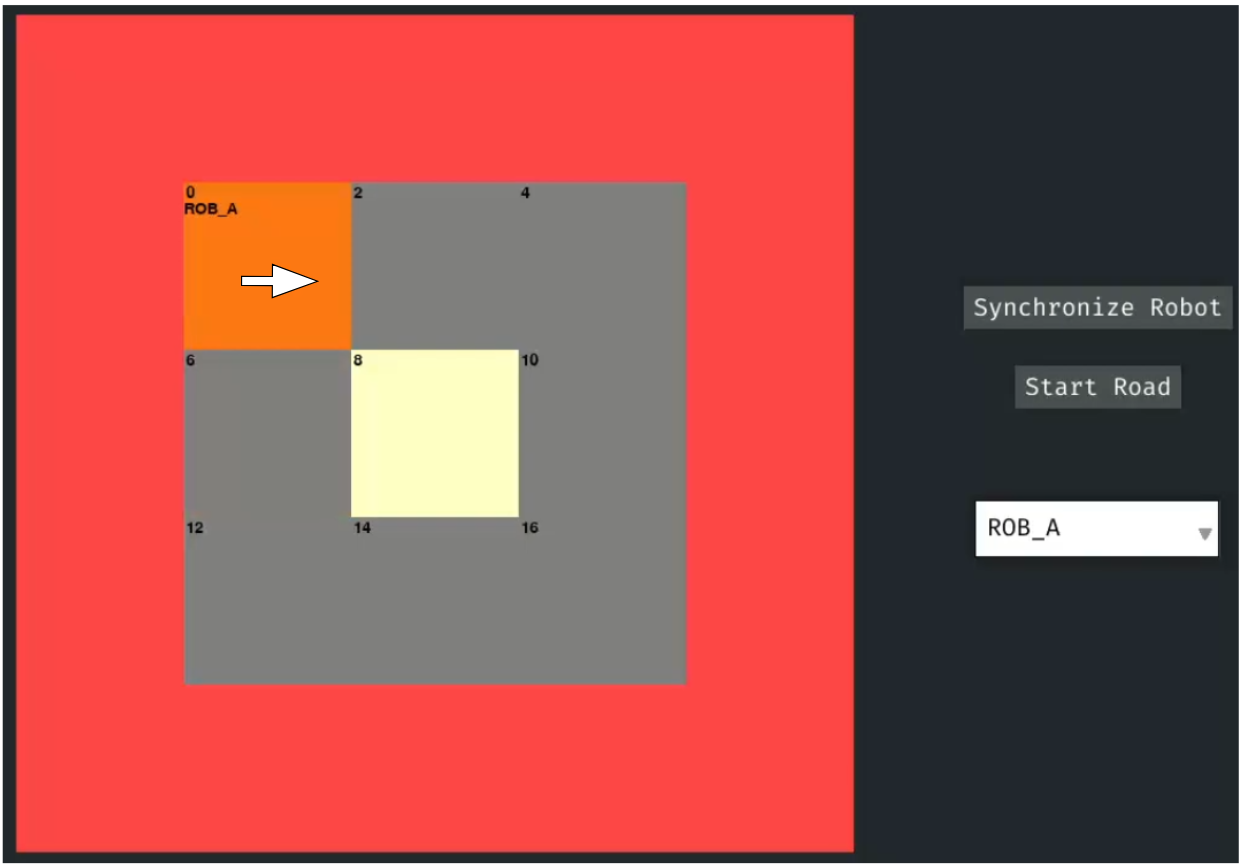
\includegraphics[width=1.0\linewidth]{images/integ_sistema_interfaz_python.png}
    \caption{Interfaz para monitoreo y control en tiempo real}
    \label{fig:integsistemainterfaz}
\end{figure}

Destacamos la reducción en gran medida del error en las trayectorias realizadas. Esto queda en evidencia en las representaciones gráficas obtenidas, donde la trayectoria deseada, indicada en fucsia, y la trayectoria real estimada, marcada en verde, muestran en la Figura \ref{fig:ejemplofiltrokalman} un bajo error para todos los puntos de la misma. Las métricas obtenidas para el error de estimación promedio en las trayectorias son de $\pm3cm$.

En la imagen \ref{fig:ejemplofiltrokalman} los ejes cartesianos del gráfico están expresados en $[metros]$ y la trayectoria está compuesta por la secuencia de coordenadas:

$$ [(3,3), (2,3), (1,3), (1,2), (1,1), (2,1), (3,1)] $$

\begin{figure}[htpb]
    \centering
    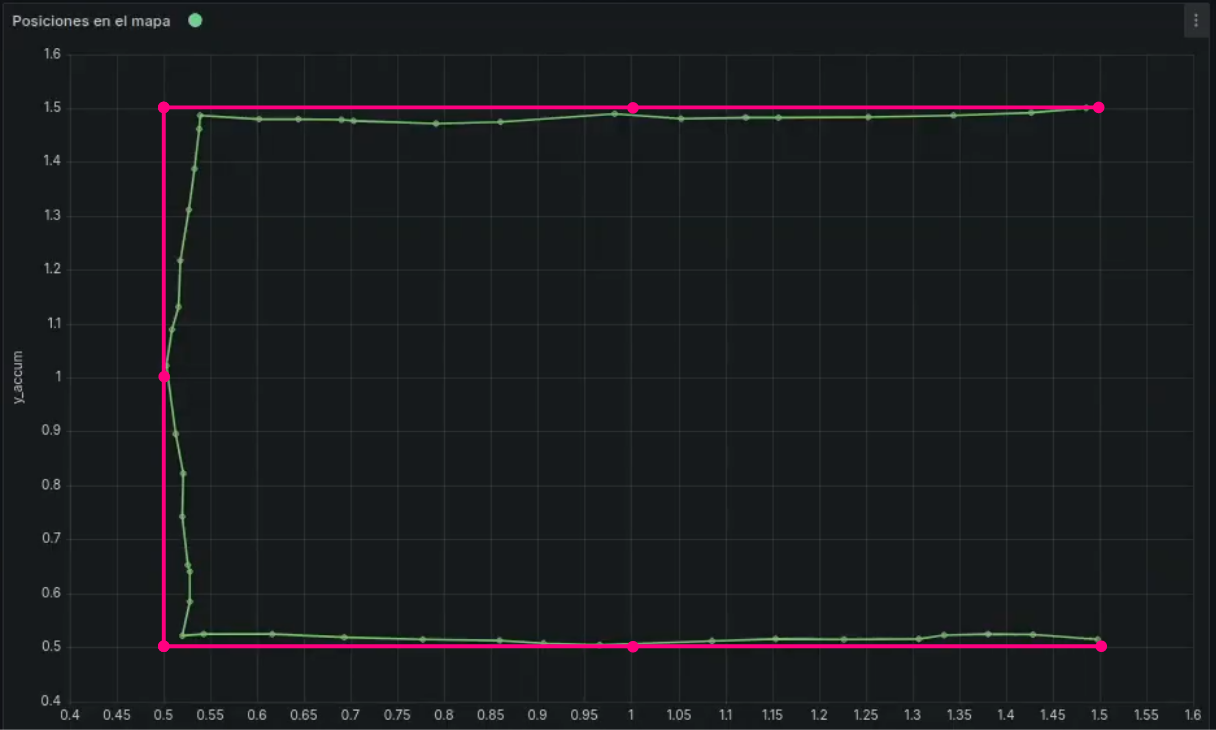
\includegraphics[width=1.0\linewidth]{images/ejemplo_trayectoria_compensacion_kalman.png}
    \caption{Ejemplo de una trayectoria realizada con el Filtro de Kalman}
    \label{fig:ejemplofiltrokalman}
\end{figure}

